\documentclass{article}
\usepackage{tikz}
\usepackage{amsmath}
\usepackage{amsfonts}
%
\begin{document}
%
% paper title
\title{ANN}
\author{Craig~Euler}
%
\maketitle
%
\begin{center}
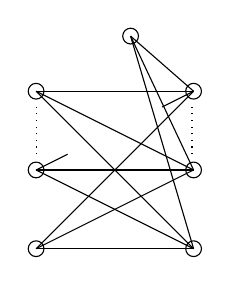
\begin{tikzpicture}
\draw (0.0, 0.0) circle (0.1cm);
\draw (0.0, 1.0) circle (0.1cm);
\draw (0.0, 2.0) circle (0.1cm);

\draw (2.0, 2.0) circle (0.1cm);
\draw (2.0, 0.0) circle (0.1cm);
\draw (2.0, 1.0) circle (0.1cm);
\draw (1.2, 2.7) circle (0.1cm);

\draw (0.0, 0.0) -- (2.0, 0.0);
\draw (0.0, 0.0) -- (2.0, 1.0);
\draw (0.0, 0.0) -- (2.0, 2.0);

\draw (0.0, 1.0) -- (2.0, 0.0);
\draw (0.0, 1.0) -- (2.0, 1.0);
\draw (0.0, 1.0) -- (0.4, 1.2);
\draw (1.6, 1.8) -- (2.0, 2.0);

\draw (0.0, 2.0) -- (2.0, 0.0);
\draw (0.0, 2.0) -- (2.0, 1.0);
\draw (0.0, 2.0) -- (2.0, 2.0);

\draw (1.2, 2.7) -- (2.0, 0.0);
\draw (1.2, 2.7) -- (2.0, 1.0);
\draw (1.2, 2.7) -- (2.0, 2.0);
\draw[dotted] (0.01, 1.2) -- (0.01, 1.8);
\draw[dotted] (1.98, 1.2) -- (1.98, 1.8);
\end{tikzpicture}
\end{center}
%
Back propagation derivation for the traditional ANN.

A caveat: the range for summation indexing is assumed from its context in these notes.
Since no absolute frame of reference will be necessary, a term such as $k \in M$ will refer to indexing over $M$ integers in $\mathbb{Z}$ ($M$ is used because $N$ will be used to refer to the number of layers in the network).

First define some shorthand $\psi_p^i$ to be the $p^{th}$ element of the result of the corresponding weights applied to the nodes at the $i^{th}$ layer along with the bias term $b^i$ and bias weight $u_p^i$:
%
\begin{equation} \label{eq:psi}
\psi_p^i = \sum_{k \in M^i} y_k^i \omega_{p,k}^i + b^iu_p^i
\end{equation}
%
Superscripts refer to the specified layer.
Hence, \eqref{eq:psi} will refer to the $i^{th}$ layer before undergoing activation.
%
where $g$ is the activation function. The sigmoid function is defined as:
%
\begin{equation} \label{eq:g}
g(x;\beta) := \frac{1}{1 + e^{-\beta x}}
\end{equation}
%
which is the activation function of choice here.
It follows that the derivative of this activation function is
%
\begin{equation} \label{eq:gp}
g'(x;\beta) = \beta \left( 1 - g(x;\beta) \right) g(x; \beta).
\end{equation}
%
Promotion to the next layer (at $i+1$) is after the activation is performed at the current layer (at $i$):
%
\begin{equation} \label{eq:z}
y_p^{i+1} := g(\psi_p^i)
\end{equation}
%
The zero-based index is used to refer to the specified layer.
For convenience (and slight redundancy with the terms $y^0$ and $y^{N-1}$), the first, interior, and last layers are denoted with $x$, $y$, and $z$ respectively.
It follows that $x = y^0$ and $z = y^{N-1}$.
Therefore, the last layer is then:
%
\begin{equation} \label{eq:z}
z_p = g(\psi_p^{N-2})
\end{equation}
%
with $N$ denoting the number of layers of the network.
%
Let the error be defined as:
%
\begin{equation} \label{eq:error}
E := \frac{1}{2} \sum_k (z_k - t_k)^2
\end{equation}
%
then
%
\begin{equation} \label{eq:derror}
\frac{\partial E}{\partial z_p} = z_p - t_p
\end{equation}
%
notice that
%
\begin{equation} \label{eq:last_layer_derror_eq_0}
\frac{\delta z_i}{\delta \omega_{p,j}} = 0, \ \ \ \forall i \neq p
\end{equation}
%
so then, at the last layer, defining the rate of change of the error term with the weights at the last layer:
%
\begin{equation} \label{eq:delta}
\delta_{i,j} := \frac{\partial E}{\partial \omega_{i,j}^{N-2}}
\end{equation}
%
\begin{equation} \label{eq:last_layer_derror}
\frac{\partial E}{\partial \omega_{i,j}^{N-2}} =
\left( \frac{\partial E}{\partial z_i} \right) \left( \frac{\partial z_i}{\partial g} \right) \left ( \frac{\partial g}{\partial \omega_{i, j}^{N-2}} \right )
\end{equation}
%
**There appears to be an error after this point. Looks like a "beta" term is missing at least**
%
\begin{equation} \label{eq:last_layer_derror3}
=
\left( z_i - t_i \right) \left( y_j^{N-2} g' (\psi_i^{N-2}) \right).
\end{equation}
%
\begin{equation} \label{eq:delta_full}
\delta_{i,j} = 
\left ( z_i - t_i \right ) y_j^{N-2} g' (\psi_i^{N-2})
\end{equation}
%
\begin{equation} \label{eq:gamma}
\gamma_{i,j} := (z_j - t_j) g'(\psi_j^{N-2})
\end{equation}
%
\begin{equation} \label{eq:gamma_array}
\gamma_i := \sum_j \gamma_{i,j}
\end{equation}
%
Expanding the derivative of the error term w.r.t. the $N-1$ layer bias weights:
%
\begin{equation} \label{eq:derive_du_nm1}
\begin{aligned}
\frac{\partial E}{\partial u_i^{N-1}} &= 
\sum_{k_{N+1}} \frac{\partial E}{\partial z_{k_{N+1}}} \frac{\partial z_{k_{N+1}}}{\partial g} \frac{\partial g}{\partial \psi_{k_{N+1}}^N} \sum_{k_N} \frac{\partial \psi_{k_{N+1}}^N}{\partial y_{k_N}^N} \frac{\partial y_{k_{N}}}{\partial g} \frac{\partial g}{\partial \psi_{k_N}^{N-1}} \sum_{k_{N-1}=i} \frac{\partial \psi_{k_N}^{N-1}}{\partial u_i^{N-1}} \\
& = \sum_{k_{N+1}} \frac{\partial E}{\partial z_{k_{N+1}}} \frac{\partial g}{\partial \psi_{k_{N+1}}^N} \sum_{k_N} \frac{\partial \psi_{k_{N+1}}^N}{\partial y_{k_N}^N} \frac{\partial g}{\partial \psi_{k_N}^{N-1}} \sum_{k_{N-1}=i} \frac{\partial \psi_{k_N}^{N-1}}{\partial u_i^{N-1}} \\
& = \sum_{k_{N+1}} \frac{\partial E}{\partial z_{k_{N+1}}} \frac{\partial g}{\partial \psi_{k_{N+1}}^N} \frac{\partial \psi_{k_{N+1}}^N}{\partial y_i^N} \frac{\partial g}{\partial \psi_i^{N-1}} \frac{\partial \psi_i^{N-1}}{\partial u_i^{N-1}} \\
& = \sum_{k_{N+1}} (z_{k_{N+1}} - t_{k_{N+1}}) (
\end{aligned}
\end{equation}
%
then
%
\begin{equation} \label{eq:delta2}
\delta_{i,j}^{N-1} =
\sum_{k_{N+1}} \delta_{k_{N+1},j}^N \omega_{k_{N+1},i}^N
\end{equation}
%
and
%
\begin{equation} \label{eq:end_weights}
\omega_{new}^N = \omega_{old}^N - \eta \delta^N
\end{equation}
%
interior weights, for $p < N$, are updated as follows:
%
\begin{equation} \label{eq:w_weights}
\omega_{new}^p = \omega_{old}^p - \eta \delta_w^p
\end{equation}
%
\begin{equation} \label{eq:u_weights}
u_{new}^p = u_{old}^p - \eta \delta_u^p
\end{equation}
%
where
%
\begin{equation} \label{eq:w_delta}
\delta_w^{q} = g'(\psi^{q}) (y^{q})^T \odot (\omega^{q+1})^T (\zeta^{q+2})^T ... (\zeta^N)^T \odot \gamma
\end{equation}
%
\begin{equation} \label{eq:u_delta}
\delta_u^{q} = g'(\psi^{q}) (b^{q})^T \odot (\omega^{q+1})^T (\zeta^{q+2})^T ... (\zeta^N)^T \odot \gamma
\end{equation}
%
where
%
\begin{equation} \label{eq:u_delta}
\zeta_{i,j}^q = \omega_{i,j}^q y_j^{\prime q} = \omega_{i,j}^q \beta (1 - y_j^q) y_j^q
\end{equation}
%
\end{document}
